% !TeX TXS-program:compile = txs:///pdflatex/[--shell-escape]
\documentclass[12pt, a4paper]{article}

% !TeX root = ../main.tex
\usepackage{a4wide}

\usepackage[utf8]{inputenc}

%\usepackage[ngerman]{babel}
\usepackage[english]{babel}

\usepackage[T1]{fontenc}
\usepackage{palatino}

\usepackage{graphicx}
\usepackage{caption}
\usepackage{url}
\usepackage{tocloft}
\usepackage{acronym}

\usepackage{mathpazo}
\usepackage{amsmath}
\usepackage{amsfonts}
\usepackage{adjustbox}

%\usepackage{subcaption}

\usepackage{hhline}
\usepackage{amssymb}
\usepackage{floatflt}
\usepackage{setspace}
\usepackage{float}
\usepackage{color}
\usepackage{listings}
\usepackage{array}
\usepackage{scrhack}
\usepackage{xcolor}
\usepackage{wrapfig}
\usepackage{hyperref}
\usepackage{url}
\usepackage{lmodern}
\usepackage{multirow}
\usepackage{subfig}
\usepackage{cleveref}
\usepackage{lipsum}


% !TeX root = ../main.tex
%%%%%%%%%%%%%%%%%%%%%%%%%%%%%%%%%%%%%%%%%%%%%%%%%%%%%%%%%%%%%%%%%%%%%%%%
% Data about you and the Document%
%%%%%%%%%%%%%%%%%%%%%%%%%%%%%%%%%%%%%%%%%%%%%%%%%%%%%%%%%%%%%%%%%%%%%%%%

% % Main Title of Document:
\newcommand{\myMaintitle}{Untersuchung und Aufbau einer DevOps Development Umgebung}

% % Sub Title of DocInput:
\newcommand{\mySubtitle}{Developing holistic software solutions through integration of existing individual solutions.}

% % Ihr Name:
\newcommand{\myName}{Henrik Gerdes}

% % Matrikelnummer:
\newcommand{\myMatrikel}{MatNr: 969272}

% % Ihr Geburtsort:
\newcommand{\brith}{Osnabrück}

% % Ihr Geburtsort:
\newcommand{\place}{Osnabrück}

% % Ihr Abgabedatum:
\newcommand{\submission}{\today}

% % Ihr Abgabedatum:
\newcommand{\mycourse}{Exposé für den B.Sc.}

% % Name des Betreuers/Erstprüfenden:
\newcommand{\fistSupervisor}{Dennis Ziegenhagen}
\newcommand{\secSupervisor}{Achim Hendrix}

% % In welchem Semester befinden Sie sich?
\newcommand{\mySemester}{6. Semester}

\title{\myMaintitle}

\author{\myName}
% !TeX root = ../main.tex
% % Zeilenabstand im Haupttext auf anderthalb-zeilig setzen
%\linespread{1.25}\selectfont

% Line spacing
%\onehalfspacing{}

%Pfad für Grafiken
\graphicspath{{fig/}}

%Styleregeln
\widowpenalty10000 % Vermeidet einzelne Zeilen eines Absatzes zu Beginn einer Seite
\clubpenalty10000 % Vermeidet einzelne Zeilen eines Absatzes am Ende einer Seite
\addtocontents{toc}{\protect\sloppy}
\setcounter{tocdepth}{3}


% % \sloppy bewirkt, dass Latex beim Blocksatz nicht über den rechten Rand hinausschreibt.
% % und dafür größere Lücken in einer Zeile in Kauf nimmt
\sloppy

% % Setzt Dokumenteigenschaften für PDFs, wenn das Paket 'hyperref' geladen wurde.
\hypersetup{pdftitle=\myMaintitle,pdfauthor=\myName,bookmarksopen=true}

%Source for picture captions
\newcommand{\source}[1]{\caption*{Source: {#1}} }

\newcommand{\code}[1]{\texttt{#1}}

\newcommand{\myparagraph}[1]{\paragraph{#1}\mbox{}\\}

\newcommand{\RM}[1]{\MakeUppercase{\romannumeral{} #1{}}}

\newcommand{\HRule}{\rule{\linewidth}{0.5mm}} % Defines a new command for horizontal


\definecolor{dkgreen}{rgb}{0,0.6,0}
\definecolor{gray}{rgb}{0.5,0.5,0.5}
\definecolor{mauve}{rgb}{0.58,0,0.82}

\lstset{ %
  language=Java,                  % the language of the code
  basicstyle=\footnotesize,       % the size of the fonts that are used for the code
  numbers=left,                   % where to put the line-numbers
  numberstyle=\tiny\color{gray},  % the style that is used for the line-numbers
  stepnumber=1,                   % the step between two line-numbers. If it's 1, each line
                                  % will be numbered
  numbersep=5pt,                  % how far the line-numbers are from the code
  backgroundcolor=\color{white},  % choose the background color. You must add \usepackage{color}
  showspaces=false,               % show spaces adding particular underscores
  showstringspaces=false,         % underline spaces within strings
  showtabs=false,                 % show tabs within strings adding particular underscores
  frame=single,                   % adds a frame around the code
  rulecolor=\color{black},        % if not set, the frame-color may be changed on line-breaks within not-black text (e.g. commens (green here))
  tabsize=4,                      % sets default tabsize to 2 spaces
  captionpos=b,                   % sets the caption-position to bottom
  breaklines=true,                % sets automatic line breaking
  breakatwhitespace=false,        % sets if automatic breaks should only happen at whitespace
  title=\lstname,                 % show the filename of files included with \lstinputlisting;
                                  % also try caption instead of title
  keywordstyle=\color{blue},          % keyword style
  commentstyle=\color{dkgreen},       % comment style
  stringstyle=\color{mauve}         % string literal style
}

%%%%%%%%%%%%%%%%%%%%%%%%%%%%%%%%%%%%%%%%%%%%%%%%%%%%%%%%%%%%%%%%%%%%%%%%%%%%%%%%%%%%%%%%%
%Examples
%%%%%%%%%%%%%%%%%%%%%%%%%%%%%%%%%%%%%%%%%%%%%%%%%%%%%%%%%%%%%%%%%%%%%%%%%%%%%%%%%%%%%%%%%
% \pdfmarkupcomment[markup=Squiggly,color=green]{with pdfcomment}{move to the front}.
% \pdfmarkupcomment[markup=StrikeOut,color=red]{stupid}{replace stupid with funny}
% \pdfmarkupcomment[markup=Highlight,color=yellow]{Of course, you can highlight complete sentences.}{Highlight}
% \pdfcomment[icon=Note,color=blue]{insert graphic!}
% Listings style file

\lstdefinelanguage{docker}{
  keywords={FROM, RUN, COPY, ADD, ENTRYPOINT, CMD,  ENV, ARG, WORKDIR, EXPOSE, LABEL, USER, VOLUME, STOPSIGNAL, ONBUILD, MAINTAINER},
  keywordstyle=\color{orange}\bfseries,
  identifierstyle=\color{black},
  % basicstyle=\small,
  sensitive=false,
  comment=[l]{\#},
  commentstyle=\color{blue}\ttfamily\emph,
  stringstyle=\color{dkgreen}\ttfamily\textbf,
  morestring=[b]',
  morestring=[b]"
}

\lstdefinelanguage{docker-compose}{
  keywords={image, environment, ports, container_name, ports, volumes, links},
  keywordstyle=\color{blue}\bfseries,
  identifierstyle=\color{black},
  sensitive=false,
  comment=[l]{\#},
  commentstyle=\color{purple}\ttfamily,
  stringstyle=\color{red}\ttfamily,
  morestring=[b]',
  morestring=[b]"
}
\lstdefinelanguage{docker-compose-2}{
  keywords={version, volumes, services, networks, image},
  keywordstyle=\color{blue}\bfseries,
  keywords=[2]{environment, ports, container_name, ports, links, build, expose, env_file, restart, depends_on}
  keywordstyle=[2]\color{olive}\bfseries,
  identifierstyle=\color{black},
  sensitive=false,
  comment=[l]{\#},
  commentstyle=\color{purple}\ttfamily,
  stringstyle=\color{red}\ttfamily,
  morestring=[b]',
  morestring=[b]"
}

\lstset{basicstyle=\ttfamily,
  inputencoding=utf8,
  extendedchars=true
  basicstyle=\footnotesize,       % the size of the fonts that are used for the code
  numbers=left,                   % where to put the line-numbers
  numberstyle=\tiny\color{gray},  % the style that is used for the line-numbers
  stepnumber=1,                   % the step between two line-numbers. If 1 = all lines numberd
  numbersep=5pt,                  % how far the line-numbers are from the code
  backgroundcolor=\color{white},  % choose the background color. You must add \usepackage{color}
  showspaces=false,               % show spaces adding particular underscores
  showstringspaces=false,         % underline spaces within strings
  showtabs=false,                 % show tabs within strings adding particular underscores
  frame=single,                   % adds a frame around the code
  rulecolor=\color{black},        % if not set, the frame-color may be changed on line-breaks
  tabsize=4,                      % sets default tabsize to 2 spaces
  captionpos=b,                   % sets the caption-position to bottom
  breaklines=true,                % sets automatic line breaking
  breakatwhitespace=false,        % sets if automatic breaks should only happen at whitespace
  title=\lstname,                 % show the filename of files included with \lstinputlisting;
  keywordstyle=\color{blue},      % keyword style
  commentstyle=\color{dkgreen},   % comment style
  stringstyle=\color{mauve}       % string literal style
}


% \pagestyle{plain}
\pagestyle{fancy}
\fancyhf{}
\fancyhfoffset[L]{1cm} % left extra length
\fancyhfoffset[R]{1cm} % right extra length
\rhead{\thepage}
\lhead{\nouppercase\leftmark}
\cfoot{\fancyplain{}{\thepage} }

\begin{document}

\pagenumbering{gobble}
% !TeX root = ../main.tex
%%%%%%%%%%%%%%%%%%%%%%%%%%%%%%%%%%%%%%%%%
% Academic Title Page
% LaTeX Template
% Version 2.0 (17/7/17)
%
% This template was downloaded from:
% http://www.LaTeXTemplates.com
%
% Original author:
% WikiBooks (LaTeX - Title Creation) with modifications by:
% Vel (vel@latextemplates.com)
%
% License:
% CC BY-NC-SA 3.0 (http://creativecommons.org/licenses/by-nc-sa/3.0/)
%
% Instructions for using this template:
% This title page is capable of being compiled as is. This is not useful for
% including it in another document. To do this, you have two options:
%
% 1) Copy/paste everything between \begin{document} and \end{document}
% starting at \begin{titlepage} and paste this into another LaTeX file where you
% want your title page.
% OR
% 2) Remove everything outside the \begin{titlepage} and \end{titlepage}, rename
% this file and move it to the same directory as the LaTeX file you wish to add it to.
% Then add \input{./<new filename>.tex} to your LaTeX file where you want your
% title page.
%
%%%%%%%%%%%%%%%%%%%%%%%%%%%%%%%%%%%%%%%%%

%----------------------------------------------------------------------------------------
%	TITLE PAGE
%----------------------------------------------------------------------------------------
%Titelseite
\begin{titlepage}
	\centering
	\thispagestyle{empty}
	\begin{center}
	
\includegraphics[width=0.9\textwidth]{uos.pdf}
	\end{center}
	\LARGE{\textsc{Institut für Informatik}}
	\vfill
	\textsc{\Large{\emph{\mycourse}}}\\[0.5cm]
	\HRule\\[0.4cm]
	\vspace{8mm}
	\huge{\textbf{{\fontfamily{ppl}\selectfont
	\myMaintitle}}}\\
	\HRule\\[0.4cm]
	\vspace{9mm}

	\begin{minipage}{0.4\textwidth}
		\begin{flushleft}
			\large
			\textit{Author}\\
			\textsc{\myName}\\ % Your name
			\textsc{\myMatrikel} % Your name
		\end{flushleft}
	\end{minipage}
	~
	\begin{minipage}{0.4\textwidth}
		\begin{flushright}
			\large
			\textit{Supervisor}\\
			\textsc{\fistSupervisor}\\ % Supervisor's name
			\textsc{\secSupervisor} % Supervisor's name
		\end{flushright}
	\end{minipage}

	\vspace{5cm}
	\large{\today}
	\vfill
	\end{titlepage}
	\newpage

% For printing add this
\newpage\null\thispagestyle{empty}\newpage

% Title & Abstract
\maketitle
\begin{abstract}
    \textbf{English:} \lipsum[20]
\end{abstract}
\begin{abstract}
    \textbf{German:} \lipsum[20]
\end{abstract}
\newpage

% Table of Contents
\tableofcontents
\newpage

% Normal page numbering
\newcounter{lastroman}
\setcounter{lastroman}{\value{page}}
\pagenumbering{arabic}

% Line spacing
% \onehalfspacing{}

\section{Introduction}\label{sec::intro}
Digital service solutions are becoming more and more relent and popular as a result of the ever-increasing possibilities and availability of technology. Due to the COVID-19 pandemic new remote working tools, digital education resources, a connected healthcare system and seamless (video) communication systems are needed. The ecommerce marked grew by 32\% up to sales volume of \$791.70 \cite{online_shopping_inc} and the overall revenue in the software market ist expected to grow from 532 billions (2020) to 772 Billion in 2025 \cite{software_industry_groth}. The need for digital business solution is bigger than ever before. To provide fast and suitable software solutions developers need adequate development setups, also called development environments. This thesis analysis modern agile software development environments, points out potential problems and purposes a virtualized software development solution to improve decelopment efficiency.\newline
This Section provides an overview about this thesis. It will briefly describe the fundamental core question of this thesis, point out its relevance and presents a possible solution approach. Subsequently, a clear delineation is then given as to what is and is not covered in this thesis. The last Section of the introduction gives a structural overview of how the thesis is structured and how it will approach the given problem.
    \subsection{Structural Overview}
    This Section gives an initial overview and delineation to this thesis. Following this Section, there is a description of the main topic of this work and the goal that should be achieved. Section \ref{sec::backgrund} provides overall background information, which are recommended for further understanding. Common and modern development methodologies are described in Section \ref{ssec::devops}, followed by Microservice and container basics in Section \ref{ssec::microservices} and \acl{CI} tools in \ref{ssec::ci_cd}. In Section \ref{sec::problem} will be a detailed analysis of current development setups and the problems encountered in these setups. The problems are illustrated with examples and their consequences for the development process, the overall project and its quality, which is emblematic of user satisfaction, are presented. Section \ref{sec::solution_concept} proposes a conceptual solution, defines its usability and workings while also providing conditions and limitations for such a solution. This solution concept is applied in Section \ref{sec::solution_code} by implementing it in a practical reference project. The implementation process is described and additional challenges and tricks for practical use are presented. Section \ref{sec::eval} discusses the proposed solution and shows its strengths and weaknesses. At the end, an outlook on future application areas and alternative solutions is given in Section \ref{sec::outlook}, followed by the conclusion in Section \ref{sec::conclusion}.

    \subsection{Problem Description}
    The rise of Agile development and Microservices was accelerated by the emergence of new technologies that changed the way \textit{where} and \textit{how} software is running. Applications could be distributed and scaled quickly through the cloud which benefited customers favors for quick changes. Yet the actual coding setup has not changed significantly.\newline
    Requirements for development environments differ depending on the project type. The development process of (\acs{GUI}) applications for PC's and smartphones is quite different to web-services development. As the functionality of web services continues to grow, while being a cost-effective way to deliver across platforms products, this method is becoming increasingly popular. However, the operating system used for the development process often differs to the operating system used to run these applications in production. This can cause platform dependent errors. Managing language runtime versions between team members or different projects become a challenge, as these can lead to unexpected program behavior or result in library version conflicts. The usage of a \acl{MSA}, due to its easy scalability, adaptability and rapid development, brings further problems. Microservices require additional configuration effort and increases the difficulty level for whole system tests, also called end-to-end tests. The initial setup for new developers can get quiet complex, requires time and might even discourage developers in open source projects.\newline
    These characteristics add additional effort, can introduce new errors and slow down the development speed, resulting in higher cost and lower customer experience.

    \subsection{Scope of the Thesis}
    The range of different software development environments is large and differs significantly from each other depending on the project. Since the development of web-based solutions is becoming more and more popular, priority is given only to these types of projects. Native application development for PCs and smartphones, as well as the development of embedded systems and other hardware-related solutions are not covered in this thesis.\newline
    In particular, the solution concept shown is not a general solution that is a perfect fit for all projects and therefore is not generally transferable. It is intended only as a solution template that contains many tricks for dealing with the problems described in Section \ref{sec::problem}. Although Section \ref{sec::backgrund} offers an explanation of fundamental topics and Section \ref{ssec::toolsused} a deeper insight into the functionality of technologies used, nevertheless not all addressed contents can be explained fundamentally. Basic knowledge of the software development process, essential programs and abstract understanding of different operating systems and network techniques are recommended.

    \subsection{Goal of the Theses}
    In the process of this work, the challenges and obstacles of modern software development environments are identified and presented. Based on these findings, a solution concept, for these challenges, is created based on virtualization technologies. The technologies used are explained, and the solution concept is applied to a reference project. Subsequently, the practicability of the solution approach is evaluated and classified. In principle, the goal of this thesis is to identify obstacles in current software development setups and to analyze the effectiveness of the proposed solution.\newpage

\section{Background Information about Agile, Container and Microservices}\label{sec::backgrund}
The following Section provides some basic definitions and principles that are necessary for the further understanding of this paper and ensures a common level of knowledge of these topics.\newline
First of will be a formal definition of DevOps, a brief description of the emergence and its current state.
    \subsection{Modern Methodologies: Agile and DevOps}\label{ssec::devops}
    This Section provides a formal definition of agile software development Paradigms and the DevOps methodology, explains their connection and points out the fundamental principles of a DevOps enabled culture. These principles and their workflows will be revisited in Section~\ref{sec::solution_concept} as part of the proposed solution concept.

        \subsubsection{Agile Development}
        Agile, just like the \wordhighlight{V-Model}, \wordhighlight{Waterfall} and \wordhighlight{Prototyping} model, is a software development paradigm. It was proposed and popularized by the \wordhighlight{"Manifesto for Agile Software Development"}, written and published in 2001 by various authors~\cite{manifesto}. Rapid adoption to changes, continuous evolution of software and customer communication are the fundamentals of agile software development.\newline
        The four core principles are:

        \begin{itemize}[label=\(\star\)]
            \setlength\itemsep{0em}
            \item \textbf{Individuals and interactions} over processes and tools
            \item \textbf{Working software} over comprehensive documentation
            \item \textbf{Customer collaboration} over contract negotiation
            \item \textbf{Responding to change} over following a plan
        \end{itemize}

        \noindent Paradigms like Waterfall describe a comprehensive model with a detailed requirements analysis and architecture design phase. This results in a fixed and detailed sequential schedule for the implementation, testing and requirements fulfillment verification phase. Errors in the requirements analysis or changes in requirements can cause difficulties later phases of the project. Agile on the other handle only provides guidelines instead of a complete model. Changes are expected and the project realization is designed to be adaptable. Project phases such as implementation and testing run together and the entire \ac{SDLC} is kept shorter and more adaptive \cite{agile_practice}.\newline
        Agile provides a mindset for projects with uncertain or continuous changing requirements. Accordingly, the agile manifesto became the foundation of several software development mythologies and frameworks that extend these fundamental guidelines and provide additional workflows and tooling for the software creation process. Well known examples are methodologies such as \wordhighlight{SCRUM}, \wordhighlight{\ac*{XP}} and \wordhighlight{DevOps}.

        \subsubsection{DevOps Definition}
        DevOps is a set of practices in software development hat aims to increase costumer value and software quality by shortening the development life cycle through active collaboration and continuous delivery of improvements \cite{base_devops}, \cite{effective_devops}. The term \wordhighlight{DevOps} is a neologism from development (Dev) and operation (Ops). The combination of these terms is symbolic for the tighter collaboration between the development and operations team, which were previously strictly separated. Therefore, DevOps is considered more than just software development principles, it is called a mindset and company/development culture. Shorter development times and closer collaboration are goals of agile software development paradigm. DevOps builds upon the guidelines and goals of agile and offers additional workflows and tools for software development to increased user experience value \cite{azuredevops}, \cite{effective_devops}.

        \subsubsection{Principles of DevOps}\label{ssec::devops_princibles}
        DevOps builds upon the agile principles. It extends the \wordhighlight{\acl{XP}} approach by also applying its principles to the operations and infrastructure aspects of the application \cite{effective_devops}. The goal is to provide a structured and comprehensive process from coding up to application monitoring. This process is referred to as a workflow and the minimal steps in an exemplary workflow are shown in table~\ref{tab::devops_steps}~\cite{base_devops}.\newline

        \begin{table}[!h]
            \centering
            \begin{tabularx}{0.85\textwidth}{llX}
                \multicolumn{2}{l}{Step} & Description \\ \hline\hline
                1 & \textbf{Coding}& Code development \& review and source control.  \\
                2 & \textbf{Building}& \acs{CI} build and build status.  \\
                3 & \textbf{Testing}& \acs{CI} testing and testing feedback.  \\
                4 & \textbf{Packaging}& Bundle and package to a central registry.  \\
                5 & \textbf{Releasing}& Release management, approvals and automation.  \\
                6 & \textbf{Configuring}& Infrastructure configuration and management.  \\
                7 & \textbf{Monitoring}& Applications performance monitoring.  \\
            \end{tabularx}
            \caption{DevOps workflow steps.}
            \label{tab::devops_steps}
        \end{table}

        \noindent With such a workflow come tasks that are the core procedures in a DevOps environment. These tasks include configuration management, release management, \ac{CI}, \ac{CD}, \ac{IaC}, test automation and application performance monitoring~\cite{azuredevops}.\newline
        For the scope of this work, only solutions from configuration management, \ac{CI} and \ac{IaC} will be used to enable a homogeneous development environment. The configuration management is about versioning the applications runtime environment and how to set it up. It determines on how the application interacts with the system and external interface services. Common configuration parameters are the compiler/interpreter version, resources and permission settings as well as domain-names or \acs{IP}-addreses of other (external) services \cite{base_devops}. A DevOps principled architecture has multiple deployment stages. A staging and live environment is considered minimal base of any such projects. Adding a local environment increases the overall amount of configuration effort, requiring a reliable, efficient way to manage it. This is closely related to the \ac{IaC} principle, which describes the provisioning process of computing resources. Tools like Ansible, Puppet and Terraform can automatically create and set up new cloud \ac{VM}s specified in a playbook. Playbooks are structured policies written in a custom language which are also stored in a \ac{VCS} \cite{ansible2020}, \cite{azuredevops}. These files describe how the host operating system is configured. Changes on these files can be handled the same way as regular code, starting with a pull request, reviews, test and approval of the changes. The \acl{IaC} principle will later be used to properly handle the setup of development containers, next to the \acs{CI} tools wich are described in Section~\ref{ssec::ci_cd}.

    \subsection{Container and Microservice Concept}\label{ssec::microservices}
    The following Section provides a basic understanding about the concepts of Microservices, how tey are implemented and what possibilities they bring with them and what limitations they have. In this context, different strategies of visualization are explained, which are also used in Section~\ref{sec::solution_concept}.

        \subsubsection{Fundamental Idea of Microservices}
        The fundamental idea of \ac{MSA} is to have small selfcontained, independently deployable software applications. Connections between these applications make it possible to provide a greater service with an extensive range of functions \cite{micro}. An exemplary structure of a microservice cluster is visualized in figure \ref{fig::micro}. It shows multiple Microservices that each expose one functionality to the outside world. Application end-points such as a \ac{UI} provide a broad function range by internally calling multiple Microservices. In the event of one application failure, only that specific functionality becomes unavailable, the remaining system keeps operational. Because of this architectural design feature is advised that, while working with data, each microservice has its own Database. This prevents having a central database becoming a single point of failure. Another core feature of Microservices in its scalability. If the load on one part of the service increases, new instances of that application can be deployed to balance to load across all instances. This concept requires a fast and reliable process to create new application instances.\newline
        The installation and setup process of new hardware can be a time-consuming task. To reduce the amount of time it takes to create new application instances, the software industry uses the concept of virtualization.

        \begin{figure}
            \centering
            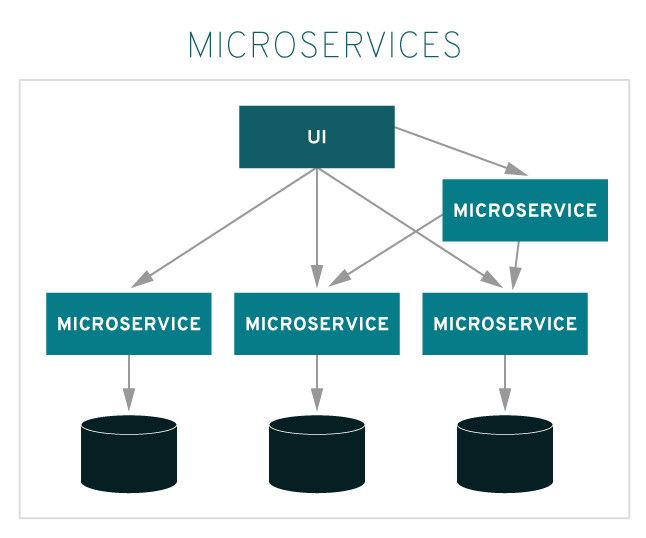
\includegraphics[width=0.5\textwidth]{monolithic-vs-microservices_altered.png}
            \caption{Structure of Microservices - [Altered], \\\textit{Source:~\cite{redhat_micro}}}\label{fig::micro}
        \end{figure}

        \subsubsection{Virtualization and Containerization}
        Virtualization is an abstraction layer. The physical hardware (called host) runs a hypervisor that allows the execution of (multiple) virtual machines (called guests) which act like a regular computer \cite{vmbasics}. This approach allows the usage of heterogeneous hardware without an impact on the guest operating systems thanks to the abstraction provided by the hypervisor. Without the need for specialized hardware and the dynamic allocation of resources, efficiency is also increased \cite{redhat_venv}. Additionally, virtual systems can be managed more easily because fundamentally they are just one big file on the host's storage device. They can be created on command, cloned and deleted without the configuration steps of a physical system. In the enterprise industry it is common to use this flexibility to start additional \ac{VM}s on high load. According to a study by the \ac{IDC} more than 80\% of data center workloads are virtualized \cite{virtualaddoption}. Virtualization also comes with the benefit of security. The majority of hypervisors strictly separate the host and the guest system. The guest system is not allowed to use the hosts resources and access its files unless it is explicitly configured to do so. Compromising a \ac{VM} does not affect the host or any other \ac{VM}s \cite{vmbasics}, \cite{redhat_venv}.\newline
        Full guest virtualization emulates a complete \ac{OS}, including the kernel, system libraries and even the majority of hardware devices. This abstraction comes with a performance penalty called overhead \cite{vmbasics}. A supposedly more lightweight approach of virtualization is called containerization. Studies by Ericsson Research, Nomadic Lab \cite{ieee_perfomance} and the Zhengzhou University \cite{zhengzhou_university} conclude in fact that container based solution provide better performance especially in disk \acs{I/O} and network \acs{I/O} bound scenarios. Containerization focuses on the isolation of one application process in a virtual runtime using control groups and namespace technologies \cite{cgroups}. Unlike \ac{VM}s, system and kernel functions are not virtualized and are passed through to the host machine. The result is a reduction of overhead and the ability to run additional application instances compared to \ac{VM}s with the same amount of compute resources. Figure \ref{fig::vm_docker} visualizes these differences between these approaches. The left side shows a traditional \ac{VM} based approach, on top of the host \ac{OS} runs a hypervisor which provides three full guest \acl{OS}s each with one application. Each gust is fully isolated and with its own kernel, \ac{OS} and runtime libraries. The container based solution only needs the host \ac{OS} and provides multiple application instances with shared libraries and runtimes in separated, isolated namespaces.\newline
        Apart from the performance benefits, the presumably main advantage of containers is their scalability~\cite{cintainer_scale}. Which makes them an adequate fit for Microservices. The most popular container based virtualization solutions are Docker, Podman and LXC.

        \begin{figure}
            \centering
            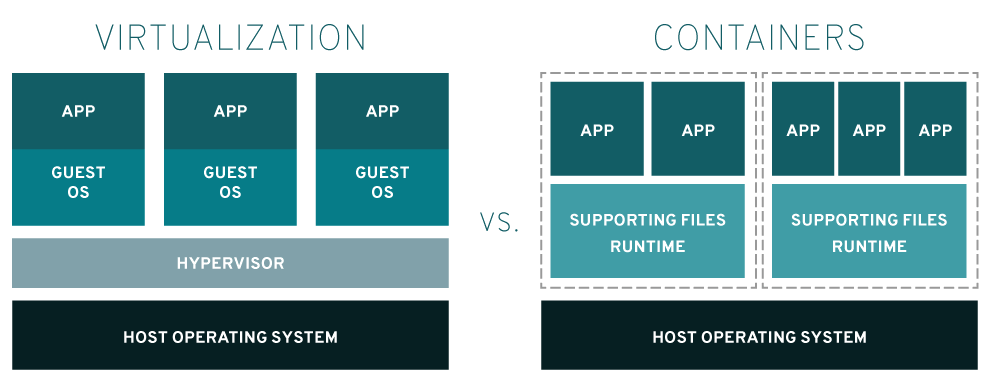
\includegraphics[width=0.9\textwidth]{docker-vm-redhat.png}
            \caption{\ac{VM}s compared to Containers, \\\textit{Source:~\cite{redhat_pic}}}\label{fig::vm_docker}
        \end{figure}

        \subsubsection{Usage of Containerization in Microservices}
        As described above, microservices are small applications that communicate with each other. To follow the principles for loose coupling between the applications the communication should be performed over a programming language independent protocol. Typical \acs{IP} network protocols used are \ac{REST}, WebSockets or GraphQL \cite{micro}. These loose coupled applications have the advantage that they can be development simultaneously from different teams as well as upgraded and replaced independently. As a result, applications can be developed much faster and more flexibly, following the principles of agile development \cite{micro}, \cite{redhat_micro}.\newline
        The usage of containers brings this speed and flexibility even further. Containers provide a consistent, isolated yet flexible runtime for applications \cite{micro_container}. Applications are packaged within known good runtimes. This reduces the setup time of the deployment and eliminate host specific errors. New application instances can be started without additional configuration. As a result of the successful concepts, tools like Docker Swarm and Kubernetes have been developed that can scale distributed applications in a managed dynamic, even automatic way.\newline
        \noindent Packaging and eventually even deploy the application introduces additional work for developers that was previously the task of the operations team. As already stated above, the developer and operations team are not separated in a DevOps culture. The new focus places value on team communication, flexibility and autonomy provided by the automation and support of as many steps as possible between the development and operation workflow \cite{effective_devops}. Eliminating manual tasks allows developers to focus on the actual application development. One of the main concepts in this process is the usage of \ac{CI} and \ac{CD} workflows.

    \subsection{Continuous Integration and Continuous Delivery Concepts}\label{ssec::ci_cd}
    \acl{CI} and \acl{CD} are two working concepts that are particularly well known in \ac{MSA}. Since every service provides only one part of the overall application functionality, it is uncertain what effects a change in one service has to other services and the wohle application.

    \subsubsection{\acl{CI}}
    \acl{CI} is a practice where new code is regularly integrated into the main code branch. Instead of having isolated functional branches that are worked on independently for months, changes flow back regularly into the main code branch to ensure it is free from conflicts and errors. Especially in interconnected services, it is indispensable to ensure that a change in one service do not have an unintended effect on other services. \ac{CI} systems can perform automatic tasks, called jobs, on the code when it is checked into the repository. These tasks can ensure a specific code-style, run Unit/\acs{API}-tests and can also run integration tests against other services. If a task fails, the corresponding developer is notified and the changes are not incorporated into the main development branch. In case of an error it becomes easier to identify the source error, due to these small and continuous integrations. Accordingly, errors and their causes can be identified more quickly and resolved without delay \cite{azuredevops}.\newline
    Popular services that provide \acl{CI} functionality are \wordhighlight{Jenikns}, \wordhighlight{Travis}, \wordhighlight{CircleCI}, \wordhighlight{GitLab \ac{CI}} and \wordhighlight{GitHub Actions}. These services differ in their function range, type of job configuration, the level of control, whether they can be self-hosted and the pricing models respectively the number of free jobs.

    \subsubsection{\acl{CD}}
    \acl{CD} on the other hand is a practice to bring these regular updates quickly and automatically into production. To ensure product quality, it is best to have multiple deployment environments, as described in Section~\ref{ssec::devops_princibles}. Each new version is automatically deployed to a test or development environment where it undergoes automatic or manual testing. Common test types are secirety scans, load- usability- and acceptence tests. If all tests are successful, the version is promoted to the next deployment environment. In case of an error, the version is discontinued, and the developers are notified about it. Only if all previous environments have not revealed any errors, the version will be transferred to production as a new release. \ac{CD} is an extension of the \ac{CI} principle and performs the next logical step in the software development workflow, accordingly \ac{CI}/\ac{CD} are often used together \cite{azuredevops}.\newline
    Figure~\ref{fig::cd} visualizes a complete exemplary \ac{CI}/\ac{CD} pipeline. It is typically built from multiple stages, where each stage bundles one or more related tasks. A stage gets triggered by an event like code check-in or a previous a previously successful stage. Common tasks are code style tests along unit tests, automatic compilation or packaging and the deployment to a test system.\newline
    Both \ac{CI} and \ac{CD} are practice to automate tasks that have previously been performed manually. Integration testing and packaging have both moved to a dedicated, autonomous system, giving developers and operators more time for other activities.
    % !TeX root = ../thesis_main.tex
\begin{figure}[]
    \centering
    \tikzstyle{block} = [rectangle, draw, fill=green!80!blue!70,
    text width=5em, text centered, rounded corners, minimum height=4em]
    \tikzstyle{line} = [draw, very thick, color=black!50, -latex']

    \begin{tikzpicture}[scale=2, node distance = 5cm, auto]
        % Place nodes
        \node [block] (init) {Code Check-in};
        \node [block, right of=init] (test) {\ac{CI} Pipeline \& Code-Test};
        \node [block, right of=test] (build) {Build \& Package Code};
        \node [block, below of=build, node distance=3.5cm] (d_test) {Deploy to Testing};
        \node [block, left of=d_test] (d_staging) {Deploy to Staging};
        \node [block, left of=d_staging] (d_live) {Deploy to Production};

        % Draw edges
        \path [line] (init) -- node {Triggers} (test);
        \path [line] (test) -- node {If successful} (build);
        \path [line] (build) -- node [left]{If successful} (d_test);
        \path [line] (d_test) -- node [above]{If successful} (d_staging);
        \path [line] (d_staging) -- node [above]{If successful} (d_live);
    \end{tikzpicture}
    \caption{\acl{CD} Workflow, \\\textit{Source: Modeled after~\cite{azuredevops}}}
    \label{fig::cd}
\end{figure}
    \newpage

\section{Analysis of the current State of Development Environments}\label{sec::problem}
The following Section will display the current status of a typical \ac{DevEnv}, point out its problems and provides approaches for possible solutions.

    \subsection{Current State of Developer Environments}
    Software development involves a broad variety of tasks. Depending on the project, tasks can range from pure web development, desktop or mobile application development, embedded system development or the pure maintenance of one of these variants. Each of these software development fields has its own workflows and requirements for the actual development setup. Even within these specialties, there are different requirements, depending on the scope, size, power and general capability demand for the project. Accordingly, development environments setups can differ greatly from one another. In order to limit the problem scope and possible solutions, this work will only refer to web services that are built on a Microservice architecture.\newline
    Despite the increasing use of web-based \ac{IDE} such as \wordhighlight{CodeSandbox}, \wordhighlight{StackBlitz} \wordhighlight{Codespaces} and \wordhighlight{Gitpod}, native development environments are still primarily used. This is also shown by the StackOverflow Survay, according to which Windows is also the operating system primarily used by professional developers, followed by MacOS and Linux~\cite{stackoverflow2021}. Accordingly, developers need a modern computer on which all the required applications must be installed and set up locally. Depending on the application area, this may include some applications for which license costs may have to be paid and which must also be kept up to date after the initial installation. These are necessary processes in software development, but they can cost a lot of time and effort and therefore money, especially if there are many or frequently changing developers. Such a working environment gives developers a lot of control over their development environments, in contrast to the functionally restricted web-based environments, but brings effort and also many error-pronenesses as the next section shows.

    \subsection{Common Issues in Modern Development Setups}
    % \textit{Notes for me:}
    % \begin{itemize}
    %     \setlength\itemsep{0em}
    %     \item Lokale Entwicklung
    %     \item API Poking
    %     \item AWS vs local
    %     \item Unit tests
    %     \item CI Tests
    %     \item End to end tests
    %     \item Zeit/Kosten
    %     \item Config aufwand. Fokus auf code nicht auf config.
    %     \item Reproduzierbakeit
    %     \item Umgebung ist managbar
    % \end{itemize}
        \subsubsection{Missing End-to-End Test Possibilities}
        \subsubsection{Configuration Shift}
        \subsubsection{Dependency Management}
        \subsubsection{Issues Caused by Heterogeneous \acs{DevEnv}'s} % OS specific errors
        \subsubsection{Additional Effort for Developers}
    \subsection{Propsed Solution}

\section{Solution Concept of DevContainers}\label{sec::solution_concept}
    \subsection{Pre-requirements for DevContainers}
    \subsection{Description of a Conceptual Environment}
    \subsection{Available Tools and Functionality of the Technologies Used}\label{ssec::toolsused}
    The following Section provides a deeper dive technologies that implement the above concepts and why they are chosen. These inner workings are relevant for later chapters as they have a direct influence on the development of the solution concept.
        \subsubsection{Docker}
        Docker is the currently most popular containerization platform that is supported on Linux, Windows and MacOs~\cite{docker_share}. It utilizes the hosts Linux kernel and its cgroups functionality for resource isolation. On none Linux host systems Docker virtualizes the kernel via a hypervisor. Docker was chosen for its wide usage, extensive documentation and its platform independency, which enables it usage in local and productive operation.\newline
        Docker allows the isolated execution of applications within a container in a well-defined state without affecting the host. The initial state of a container is defined in a disk image that bundles all the software, libraries and configuration files needed. Images are build based on a \wordhighlight{Dockerfile} that contains sequential, imperative instructions on how the container \ac{OS} should be configured. An exemplary Dockerfile can be found in appendix in Listing \ref{code::docker}. Common steps are the \code{COPY} command to add filres form the host to the container and the \code{RUN} command to execute shell commands within the container. Each instruction that changes files adds another layer to the overlay-filesystem that is used by Docker. Effectefly makling each layer a read only filesystem once it is written. At runtime a file-lookup is performed in the top filesystem layer, if the file is not found lookups in the layers below follow. This allows the reuse of layers, because changed versions of a file are simply pushed into a new layer and overshadow the original files. Docker images are distributed via a Registry to other systems. The company that develops Docker also provides a public official Docker Image Registry called DockerHub that provides official images of common software such as databases and webservers as well as base images for own projects \cite{docker2020}, \cite{dockerdocs}.\newline
        When a container is started, the program specified in the image is executed, and the container runs until it is stopped. Each container is treated as an independent full-fledged computer with its own \ac{OS}. For this reason, each container also has its own \acs{IP} address and is by default not reachable from the host computer. The user has explicitly expose a container port to the host system in order to access the application inside the container. Each container not only has its own \acs{IP}, but is also on its own software defined network, which is managed by Docker and even provides an internal \ac{DNS} server. Containers within a defined network can communicate with each other by their names and provide their functionality outside the network by exposing their published ports to the host \ac{OS} \cite{docker2020}.\newline
        Unlike \ac{VM}s, the containers guest \ac{OS} is not maintained, as containers are considered disposable. Instead of updating the software within the container, it is simply replaced by a newer one from an updated image. All changes and new files within the container will be lost. To avoid losing user data, private keys and the like, these can be stored on the host system for persistence and made available in the container via mounts. A mounted directory behaves like new top layer in the overlay file system. Docker distinguishes between volume mounts and bind mounts. Volumes are managed by Docker, have a unique name, can easily be shared between containers and are transferable between hosts. With bind mounts a specified directory from the host is mounted to the container. All file system attributes and file properties are passed to the container, the management is done by the user \cite{docker2020}, \cite{dockerdocs}.
        \subsubsection{\ac{VCS}, \acl{CI} and \acl{CD}}
        A \acl{VCS} (\ac{VCS}) is an essential tool in the software development industry to keep track of which change was made when and by whom. Git became the defacto standard over the last 10 years and is used in this project just like by over 93\% of all developers according to the StackOverflow Developer Survay 2021~\cite{stackoverflow2018}. Git allows collaborative, distributed work in own branches without affecting others. Changes can be merged back into the main branch after an optional review and made available fall all developers. A selfhosted instance of GitLab is used to coordinate teamwork, serves as a central code repository and for task management. Its adaptability, extensive integration options and built-in \ac{CI} tools provide all the necessary software lifecycle programs from a single service. Its \ac{CI}/\ac{CD} functionality is used to automatically test, build and deploy the code to a testing environment. The built-in private container registry allows the creation of always up-to-date Docker images and make them accessible to the developers, so that this task does not burden the local computers. Alternatives are \wordhighlight{GitHub} and \wordhighlight{Bitbucket}, both of which offer code hosting, issue managment, \ac{CI} and \ac{CD}. Standalone solution for \ac{CI}/\ac{CD} are \wordhighlight{Travis}, \wordhighlight{CircleCI} or \wordhighlight{Jenikns}.
        \subsubsection{Editors}
        Editors are the primary working tool of developers when writing code. The variability and the number of different editors is great. Well known examples are Visual Studio, XCode, Atom, Sublime, Eclipse, Emacs and VIM to just name a few. There is usually a distinction between simple text editors and \acl{IDE}. While text editors are quite simple and only provide basic functionalities like syntax highlighting, \ac{IDE}s are much more comprehensive with powerful Intellisense suggestions, built-in project management, \ac{VCS}, debugger, graphical representations and buildtools. The choice of the editor is a personal decision for most developers, and they are customized according to their preferences. For this reason, this work does not require a specific editor for DevContainers, but gives a recommendation that will be used for the rest of the work.\newline
        \ac{VSCode} is a free platform independet editor from Microsoft with extensive extendabiliy wich is used by over 70\% of all developers on StackOverflow~\cite{stackoverflow2021}. One of its key beneficial features for virtualized work environments is its Remote Development function. This, officially provided, extention provides the comfort of a graphical \ac{UI} while running the code, the application and auxiliary processes like debugger on another machine. As Figure \ref{fig::vscoderemote} shows, \ac{VSCode} connects to the remote machine, installs a server instance of the editor that manages access to the file system and the execution of other processes, and communicates with the local \ac{VSCode} instance for comfortable access to these functions \cite{vscodedevcontainer}. The functionality to make remote processes available locally via port forwarding is useful to allow the usage of local programme with these remote services. This type of remote development works for \acs{SSH} connections, the \ac{WSL}, and on containers. \ac{WSL} is a feature to provid a Linux envorment on Windows without the need of a full \ac{VM}. The implementation of Docker for Windows is build upon this functionality. Details on the use and configuration of this function are described in detail in Section \ref{ssec::imp_process}. All these functions can be used without \ac{VSCode} by using remote filesystem mounts, portforwording or terminal editors, but it requires more configuration effort.
        \begin{figure}[]
            \centering
            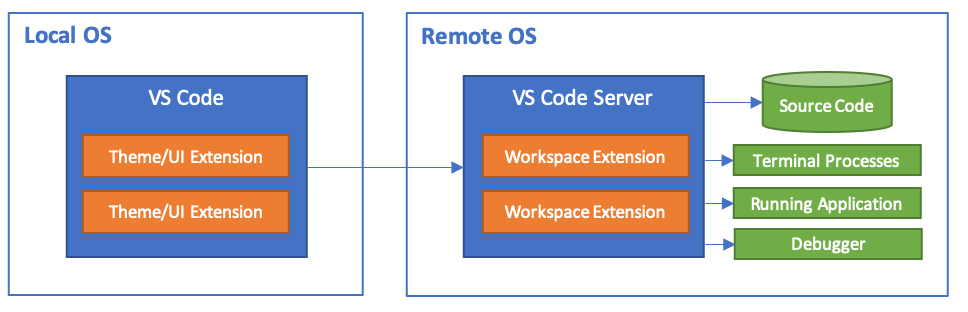
\includegraphics[width=.95\textwidth]{vscode-remote.png}
            \caption{Structure of \ac{VSCode} remote Development setup \\\textit{Source:~\cite{vscodedevcontainer}}}\label{fig::vscoderemote}
        \end{figure}
        \subsubsection{Other}
        In addition to the tools mentioned above, other auxiliary programmes are used. The use of scripts is intended to simplify the work and make recurring tasks easier. \wordhighlight{Bash} scripts can be used natively on Linux and MacOS, the installation of Git also brings Bash support to Windows. This allows operations to be performed on multiple repositories, initial settings to be set and complicated build instructions to be simplified. \wordhighlight{Docker Compose} follows the same approach and facilitates the managment of multiple interrelated Docker projects. It is a program for orchestrating multiple Docker services. It ensures that interdependent services are started in the correct order and that all necessary persistent volumes are created \cite{docker2020}, \cite{dockerdocs}. The configuration for the orchestration with compose is typically specified in a \code{docker-compose.yml} file that follows the \ac{IaC} principle and is also tracked in \ac{VCS}. An optional feature is to further organise the logs from the docker containers. Although Docker Compose offers colour-grouped log outputs per container, these can also become overwelming if there are many containers. Since the Docker stack is used anyway, enterprise log aggregators and analysis tools like \wordhighlight{Grafana} or \wordhighlight{Elastic Search} can also be used to get a persistent and personalised log dashboard. In this concept, a Grafana container is used that gets its logs from the \wordhighlight{Loki} logshipper via a Docker plugin.

    \subsection{Possible Implementations}
    \subsection{Strengths, Weaknesses and Limits}\newpage

\section{Exemplary Prototype Implementation}\label{sec::solution_code}
    % !TeX root = ../thesis_main.tex
\begin{figure}[]
    \centering
    \tikzstyle{block} = [rectangle, draw, fill=green!80!blue!70,
    text width=5em, text centered, rounded corners, minimum height=4em]
    \tikzstyle{line} = [draw, very thick, color=black!50, -latex']

    \begin{tikzpicture}[
        align=center,
        scale=0.2,
        node distance=3.5cm,
        auto]

        % Frontend
        \node [] (user) {
\includegraphics[width=.08\textwidth]{fig/user.png}\\User};
        \node [block, left of=user, xshift=-15mm] (webapp) {
\includegraphics[width=.5\textwidth]{fig/vue.png}\\WebApp};

        % Microservice Cluster
        \node [block, below of=webapp, xshift=-20mm, yshift=-5mm] (authbackend) {
\includegraphics[width=.4\textwidth]{fig/php.png}\\Auth-Backend};
        \node [block, below of=webapp, xshift=20mm, yshift=-5mm] (deviceapi) {
\includegraphics[width=.7\textwidth]{fig/node1.png}\\System-API};
        \node[draw,dashed,fit=(authbackend) (deviceapi), label={[above]MS\\Cluster}] (microcluster) {};

        % MQTT Service
        \node [block, right of=deviceapi, xshift=2mm] (mqttcon) {
\includegraphics[width=.7\textwidth]{fig/node1.png}\\MQTT Connector};
        \node [block, right of=mqttcon, xshift=7mm] (mqttbroker) {
\includegraphics[width=.3\textwidth]{fig/mqtt-logo-small.png}\\MQTT Broker};
        \node[draw,dashed,fit=(mqttbroker) (mqttcon), label={[above]MQTT\\Service}] (mqttservice){};

        % DB Stuff
        \node[database,label=below:SQL\\User \acs{DB},database radius=.8cm,database segment height=0.42cm, below of=authbackend] (userdb) {};
        \node[database,label=below:Logs\\Mongo\acs{DB} ,database radius=.8cm,database segment height=0.42cm, below of=webapp, yshift=-38mm] (logdb) {};
        \node[database,label=below:SQL\\Device \acs{DB},database radius=.8cm,database segment height=0.42cm, below of=deviceapi] (devicedb) {};

        % Device
        \node [below of=mqttbroker] (device) {
\includegraphics[width=.1\textwidth]{fig/device.png}\\Devices};

        % Edges & Paths
        \path [line] (user) -- node [text width=2.5cm, align=center, above]{Interacts\\with} (webapp);
        % To APIs
        \path [line] (webapp) -- node [text width=3.5cm, align=center, left, yshift=3mm, xshift=4mm]{Validates Authentication} (authbackend);
        \path [line] (webapp) -- node [text width=4cm, align=center, right, yshift=3mm]{Provides Device Data \& Functionality } (deviceapi);
        % To DB
        \path [line] (authbackend) -- node [text width=2cm, align=center, left, yshift=-2mm]{Connects to} (userdb);
        \path [line] (authbackend) -- node [text width=1cm, above,xshift=10mm, yshift=-5.5mm]{Event Logs} (logdb);
        \path [line] (deviceapi) -- node [text width=1cm, above, xshift=-3.5mm, yshift=-1mm]{} (logdb);
        \path [line] (deviceapi) -- node [text width=2cm, align=center, right, yshift=-2mm]{Connects to} (devicedb);
        % MQTT Device
        \path [line ] (microcluster) -- node [align=center, above] {Uses} (mqttservice);
        \path [line ] (mqttcon) -- node [text width=2cm, align=center, above] {\acs{REST} API for} (mqttbroker);
        \path [line,transform canvas={xshift=2mm}] (device) -- node [text width=2.5cm, align=center, right]{} (mqttbroker);
        \path [line, transform canvas={xshift=-2mm}] (mqttbroker) -- node [text width=3cm, align=center, left, yshift=-3mm]{Subscribe\\\& Publish\\Messages} (device);

    \end{tikzpicture}
    \caption{IoT Web Service Architecture}\label{fig::arch}
\end{figure}


    % !TeX root = ../thesis_main.tex
% \subsection{Figure Alternatives}
\begin{figure}[!h]
    \centering
    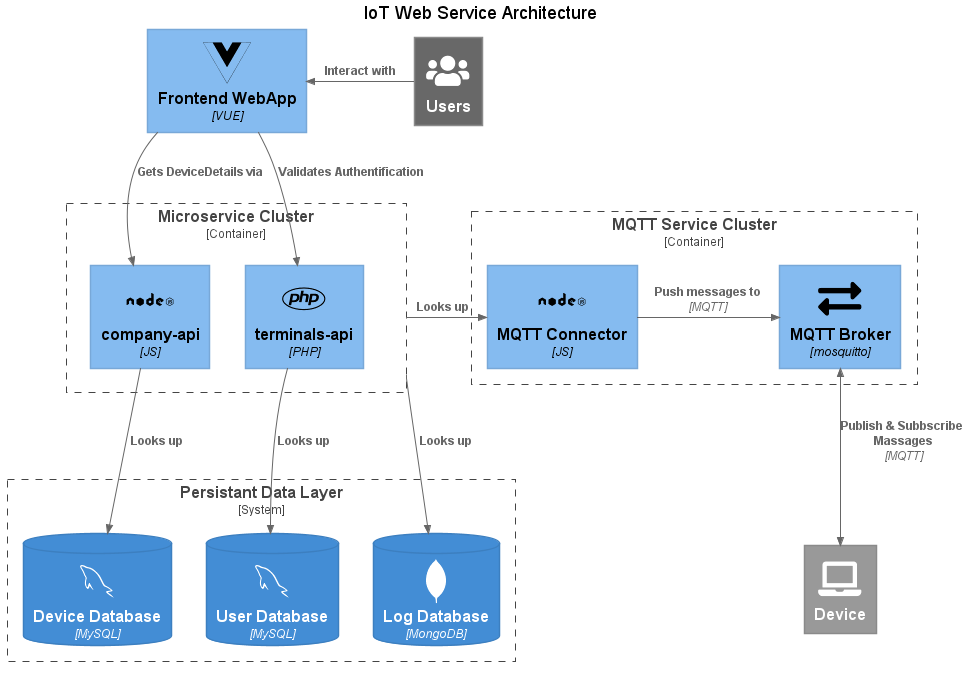
\includegraphics[width=.95\textwidth]{CCI-System-clean.png}
    \caption{IoT Web Service Architecture - [Alternative]}\label{fig::arch}
\end{figure}
    \subsection{Current State and Goal}
    \subsection{Implementation Approach}\label{ssec::imp_approach}
    \subsection{The Implementation Process}\label{ssec::imp_process}
    \subsection{Encountered Challenges and Limits}
    \subsection{Final State}
%     \begin{lstlisting}[language=bash, frame=single, backgroundcolor=\color{codebg}]
% Here is the codes format i want to show in latex
%     \end{lstlisting}


\section{Performance Evaluation and Analysis}\label{sec::eval}
\subsection{Metrics and how to Evaluate}
    \subsection{Evaluation and Results}
    \subsection{Discussion of Evaluation}

\section{Future Potential and Outlook}\label{sec::outlook}
\section{Conclusion}\label{sec::conclusion}

% STATS
% 5000 Words
% 28.300/33.200 Characters

\newpage
% Anhang
\lhead{Appendix}
\renewcommand{\thesubsection}{\Alph{subsection}}
\pagenumbering{Roman}
\setcounter{page}{\value{lastroman}}
\section*{Appendix}
\addcontentsline{toc}{section}{Appendix}

%Abkürzungsverzeichnis
% !TeX root = ../main.tex
\newcommand{\abbr}{Abbreviations}
\subsection{Abbreviations}
%\addcontentsline{toc}{subsection}{Abbreviations}

\begin{acronym}[1234567890]		%[längste Abkürzung]
\setlength{\itemsep}{-\parsep}	% sorgt dafür, dass das Verzeichnis kompakt dargestellt wird.

\acro{BLEST}[BLEST]{BLock ESTimation}
\acro{CWND}[CWND]{Congestion Window}
\acro{DAPS}[DAPS]{Delay-Aware Packet Scheduler}
\acro{ECF}[ECF]{Earliest Completion First}
\acro{HTTP}[HTTP]{Hypertext Transfer Protocol}
\acro{ISP}[ISP]{Internet Service Provider}
\acro{IETF}[IETF]{Internet Engineering Task Force}
\acro{LRF}[LRF]{Lowest-RTT-First}
\acro{MSS}[MSS]{Maximum Segment Size}
\acro{MPTCP}[MPTCP]{Multipath TCP}
\acro{MPTCPSW}[MPTCP\textsubscript{SW}]{MPTCP's send window}
\acro{OTIAS}[OTIAS]{Out-of-Order Transmission for In-Order Arrival Scheduler}
\acro{RR}[RR]{Round Robin}
\acro{RTT}[RTT]{Round Trip Time}
\acro{SCTP}[SCTP]{Stream Control Transmission Protocol}
\acro{sRTT}[sRTT]{Smoothed RTT}
\acro{STTF}[STTF]{Shortest Transfer Time First}
\acro{TCP}[TCP]{Transmission Control Protocol}
\acro{VoIP}[VoIP]{Voice over IP}
\end{acronym}
\newpage

%Code
% !TeX root = ../thesis_main.tex

\subsection{Code Listings}
% \addcontentsline{toc}{subsection}{Code for you}
\begin{lstlisting}[language=docker, frame=single, caption={Exemplary NodeJS Dockerfile},label=code::docker]
# The base image to start from
FROM ubuntu:18

# Install nodeJS
RUN apt-get update && apt-get install -y nodejs npm

# Copy content of the HOSTS "backend" folder
# to the "app" folder in the container
WORKDIR /app
COPY backend /app

# Install all node-modules
RUN npm install

# Spcify the command that is run
# when the container is started
ENTRYPOINT [ "npm", "start" ]

\end{lstlisting}


\begin{lstlisting}[language=docker-compose-2,caption={Example docker-compose.yml},breaklines=true,label={code::compose}]
version: "2"
  services:
    web:
       build: .
       ports:
          - "5000:5000"
       volumes:
          - .:/code
          - logvolume:/var/log

    redis:
       image: redis

  volumes:
    logvolume:
\end{lstlisting}

\newpage
\listoffigures
\listoftables
\lstlistoflistings{}


%Bibliographie
\addcontentsline{toc}{section}{References}
\bibliographystyle{IEEEtranSA}
% \bibliographystyle{alpha}
\bibliography{bib/sources}
% !TeX root = ../main.tex
\section*{Declaration of Authorship}

\vspace{5cm}

~\\
I hereby declare that the paper submitted is my own unaided work. I assure that I wrote this paper without using any other means and sources than those specified. As well as the sources used literally or analogously taken from the sources identified as such.

\vspace{3cm}
\begin{flushright}

\rule{8cm}{0.2mm} \\
Signature (\myName)
\end{flushright}

\vspace{2cm}
\place, the \submission{}

\end{document}